
\section{Swap channels}

One of the major issues with direct ``onchain'' payments in a blockchain network, is that each transaction must be processed
by each and every node participating in the network, resulting in high transaction costs.
One strategy to mitigate transaction costs is to defer payments and process them in bulk. 
In exchange for reduced cost, the beneficiary must be willing to incur higher risk of settlement failure.

\subsection{A simple chequebook}

A very simple smart contract that allows the beneficiary to choose when payments are to be processed, was introduced in \cite{ethersphere2016sw3}
This \gloss{chequebook} contract is a wallet that can process cheques issued by its owner. The cheques are
analgous to those in the real-world: the issuer signs a cheque specifying a beneficiary, a date and an amount,
gives it to the recipient as a token of promise to pay at a later date. The smart contract plays the
role of the bank. When the recipient wishes to get paid, they ``cash the cheque'' by submitting it to the smart contract. The contract, after validating the signature, date and the amount specified on the cheque, transfers the amount to the beneficiary's account (see figure \ref{fig:swap-chequebook}).
%Analogously to the person taking the cheque to the bank to cash it, anyone can send the digital cheque as part of the data in a transaction to the owner's chequebook account and thus trigger the transfer.

% Agents
\def\IssuerLocal{Issuer Local Store}
\def\IssuerSwapContract{Issuer Swap}
\def\BeneficiarySwapContract{Beneficiary Swap}
\def\BeneficiaryLocal{Beneficiary Local Store}

% Message Flows
\def\Issue{Issue} \def\Cheque{Cheque}
\def\Redeem{Redeem} \def\Cheque{Cheque}
\def\Clear{Clear} \def\ETH{ETH}
\def\NW{Notify Withdrawal} \def\Msg{Log Event}
\def\ND{Notify Deposit} \def\Msg{Log Event}

% Legend 
\def\LegendOnChain{On-chain}
\def\LegendOffChain{Off-chain}

% Diagram
\begin{figure}
\centering
   
\begin{tikzpicture}[every node/.style={font=\normalsize,
  minimum height=.75cm,minimum width=1cm},]

% Matrix
\node [matrix, very thin,column sep=1.3cm,row sep=0.5cm] (matrix) at (0,0) {
  & \node(0,0) (\IssuerLocal) {};   &                         & \node(0,0) (\IssuerSwapContract) {};   & & \node(0,0) (\BeneficiarySwapContract) {};   & & \node(0,0) (\BeneficiaryLocal) {}; \\
  & & & & & & & \\
  & & & & & & & \\
  & & & & & & & \\
  & \node(0,0) (\IssuerLocal 1) {}; & \node(0,0) (\Issue) {}; & \node(0,0) (\IssuerSwapContract 1) {}; & & \node(0,0) (\BeneficiarySwapContract 1) {}; & & \node(0,0) (\BeneficiaryLocal 1) {}; \\
  & & & & & & & \\
  & & & & & & & \\
  & \node(0,0) (\IssuerLocal 2) {}; &                         & \node(0,0) (\IssuerSwapContract 2) {}; & & \node(0,0) (\BeneficiarySwapContract 2) {}; & \node(0,0) (\Redeem) {};  &  \node(0,0) (\BeneficiaryLocal 2) {}; \\ 
  & & & & & & & \\
  & & & & & & & \\
  & \node(0,0) (\IssuerLocal 3) {}; &                         & \node(0,0) (\IssuerSwapContract 3) {}; & \node(0,0) (\Clear) {}; & \node(0,0) (\BeneficiarySwapContract 3) {}; &                    ; & \node(0,0) (\BeneficiaryLocal 3) {}; \\
  & & & & & & & \\
  & \node(0,0) (\IssuerLocal 4) {}; & \node(0,0) (\NW) {}   ; & \node(0,0) (\IssuerSwapContract 4) {}; &                         & \node(0,0) (\BeneficiarySwapContract 4) {}; & \node(0,0) (\ND) {}; & \node(0,0) (\BeneficiaryLocal 4) {}; \\
  & & & & & & & \\
  & \node(0,0) (\IssuerLocal 5) {}; &                         & \node(0,0) (\IssuerSwapContract 5) {};  & & \node(0,0) (\BeneficiarySwapContract 5) {};& & \node(0,0) (\BeneficiaryLocal 5) {}; \\
  & & & & & & & \\
  & \node(0,0) (\IssuerLocal 6) {}; &                         & \node(0,0) (\IssuerSwapContract 6) {};  & & \node(0,0) (\BeneficiarySwapContract 6) {};& & \node(0,0) (\BeneficiaryLocal 6) {}; \\
  & & & & & & & \\
  & \node(0,0) (\IssuerLocal 7) {}; & \node(0,0) (\LegendOnChain) {};  & & & & & \\
  & \node(0,0) (\IssuerLocal 8) {}; & \node(0,0) (\LegendOffChain) {}; & & & & & \\
};

% Agents labels
\fill 
	(\IssuerLocal) node[draw,fill=white] {\IssuerLocal}
	(\IssuerSwapContract) node[draw,fill=white] {\IssuerSwapContract}
	(\BeneficiarySwapContract) node[draw,fill=white] {\BeneficiarySwapContract}
	(\BeneficiaryLocal) node[draw,fill=white] {\BeneficiaryLocal};

\draw [dashed] 
  (\IssuerLocal) -- (\IssuerLocal 6)
  (\BeneficiaryLocal) -- (\BeneficiaryLocal 6)
  (\IssuerSwapContract) -- (\IssuerSwapContract 6)
  (\BeneficiarySwapContract) -- (\BeneficiarySwapContract 6);

% Horizontal flows (Monetary interactions)
%\draw [-latex] (\IssuerLocal 1) -- (\IssuerSwapContract 1.west) arc(180:0:0.37cm) -- (\BeneficiarySwapContract 1.west) arc(180:0:0.37cm) -- (\BeneficiaryLocal 1);
\draw [-{Latex[length=3mm,width=5mm]}] (\IssuerLocal 1) -- (\BeneficiaryLocal 1);
\draw [-{Latex[length=3mm,width=5mm]}] (\BeneficiaryLocal 2) -- (\IssuerSwapContract 2);
%\draw [-latex] (\BeneficiaryLocal 2) -- (\BeneficiarySwapContract 2.east) arc(0:180:0.37cm) -- (\IssuerSwapContract 2);
\draw [-{Latex[length=3mm,width=5mm]}] (\IssuerSwapContract 3) -- (\BeneficiarySwapContract 3);
\draw [-{Latex[length=3mm,width=5mm]}] (\IssuerSwapContract 3) -- (\IssuerLocal 4);
\draw [-{Latex[length=3mm,width=5mm]}] (\BeneficiarySwapContract 3) -- (\BeneficiaryLocal 5);

% Flows Labels 
\fill
  (\Issue) 
    node[above] {\Issue (\Cheque)}
  (\Redeem) 
    node[above] {\Redeem (\Cheque)}
  (\Clear) 
    node[above] {\Clear (\ETH)}
  (\NW) 
    node[above, text width=2.2cm,align=center,fill=white] {\NW \\(\Msg)}
  (\ND) 
    node[above, text width=3cm,align=center,fill=white] {\ND \\(\Msg)};

% Interaction points 
\draw 
  (\IssuerLocal 1) node[minimum size=0.5cm, draw,circle,fill=red!20] {}
  (\BeneficiaryLocal 1) node[minimum size=0.5cm, draw,circle,fill=red!20] {}
  (\BeneficiaryLocal 2) node[minimum size=0.5cm, draw,circle,fill=red!20] {}
  (\IssuerSwapContract 2) node[minimum size=0.5cm, draw,circle,fill=green!20] {}
  (\IssuerSwapContract 3) node[minimum size=0.5cm, draw,circle,fill=green!20] {}
  (\IssuerLocal 4) node[minimum size=0.5cm, draw,circle,fill=red!20] {}
  (\BeneficiarySwapContract 3) node[minimum size=0.5cm, draw,circle,fill=green!20] {}
  (\BeneficiaryLocal 5) node[minimum size=0.5cm, draw,circle,fill=red!20] {}
  (\IssuerLocal 7) node[minimum height=.2cm, minimum size=0.2cm, draw,circle,fill=green!20] {}
  (\IssuerLocal 8) node[minimum height=.2cm, minimum size=0.2cm, draw,circle,fill=red!20] {};

% Vertical lifelines
\draw [-{Latex[length=3mm,width=4mm]}] (\IssuerSwapContract 2) -- (\IssuerSwapContract 3);

% Legend labels
\draw
	(\LegendOnChain) node[minimum height=.2cm] {\LegendOnChain}
	(\LegendOffChain) node[minimum height=.2cm] {\LegendOffChain};

\end{tikzpicture}
\caption{The basic interaction sequence for swap chequebooks}
\label{fig:swap}
\end{figure}

Since these digital cheques are files and can therefore be copied, care must be taken that the same cheque cannot be cashed twice. Such ``double cashing'' can be prevented by assigning each cheque given to a particular beneficiary a serial number which the contract will store when the cheque is cashed. The chequebook contract can then rely on the serial number to make sure cheques are cashed in sequential order, thus needing to store only a single serial number per beneficiary.
An alternative strategy to prevent double cashing, when repeated payments are made to the same beneficiary, is that the cheques contain the \emph{cumulative} total amount ever credited to the beneficiary. The total cumulative amount that has been cashed out is stored in the contract for each beneficiary. When a new cheque is submitted, the contract ignores cheques with amount equal to or less than the stored total, but it will transfer the difference if it receives a cheque with a higher total.

This simple trick also makes it possible to cash cheques in bulk because only the current `last cheque' need ever be processed. This achieves the reduction of transaction costs alluded to above.

Incidentally, the cumulative amount stored in the contract represents the total of all outgoing payments that have been honoured and thus the contract also serves as a credit history for the owner.

The amount deposited in the chequebook (\gloss{global balance}) serves as collateral for the cheques. It is pooled over the beneficiaries of all outstanding cheques.
In this simplest form, the chequebook has the same guarantee as real-world cheques: none. Since funds can be freely moved out of the chequebook wallet at any time, solvency at the time of cashing can never be guaranteed: if the chequebook's balance is less than the amount sanctioned by a cheque submitted to it, the cheque will bounce. This is the trade off between transaction costs and risk of settlement failure.

% Parts of this deposit can be locked (\gloss{global deposit}).
% If the frequency of issuing and the amount promised are limited,
% the global balance can be informational about the likelihood of insolvency.
% If, however, there is no restrictions on issuing and paying out cheques,
% the owner can issue cheques totalling more than what is backed
% by the chequebook's global balance. Locking, by itself, provides no further guarantees, so accepting
% cheques constitutes a risk to the beneficiary.


\subsection{SWAP accounting with chequebook}

Nonetheless, even in this simple form, the chequebook proves quite useful.
\cite{ethersphere2016sw3} introduces a protocol for peer to peer accounting, called \gloss{swap}.
\gloss{swap} is a tit-for-tat accounting scheme that scales microtransactions by
allowing service for service exchange between connected peers
(\emph{swap = swarm accounting protocol for service wanted and provided}).

In case of equal consumption with low variance over time, bidirectional services can be accounted for without any payments. Data relaying is such a service, making swap
ideally suited for implementing bandwidth incentives in content delivery or mesh networks.

\begin{center}
\begin{figure}
\begin{center}
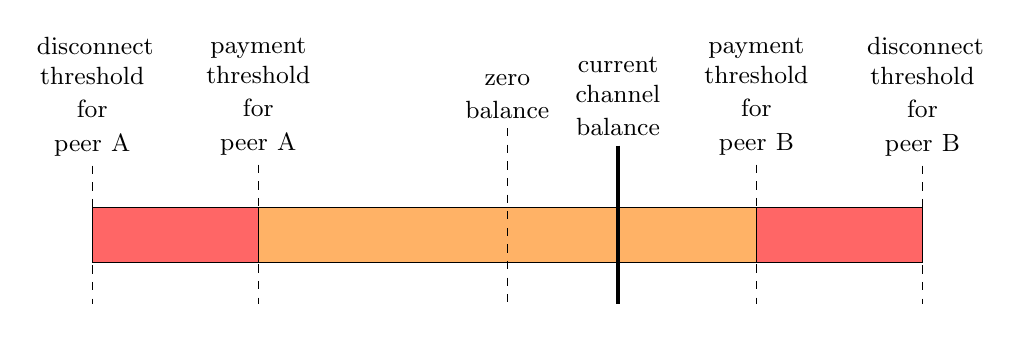
\begin{tikzpicture}
\node (middle)[draw, rectangle, fill=orange!60, minimum height=2em, minimum width=18em]{};
\node (leftred) [draw, rectangle, fill=red!60, minimum height=2em, minimum width=6em, node distance=12em,left of=middle]{};
\node (rightred)[draw, rectangle, fill=red!60, minimum height=2em, minimum width=6em, node distance=12em,right of=middle]{};
\node (zero) [above of=middle,node distance=5em, text width=4em, align=center] {\small zero\\ balance};
\node (zerod) [below of=middle] {};
\draw [dashed](zero)--(zerod);
\node (rtol) [node distance=9em,right of=zero,text width=4em, align=center] {\small payment\\threshold\\for peer B};
\node (rtold) [node distance=9em,right of=zerod] {};
\node (ltol) [node distance=9em,left of=zero,text width=4em, align=center] {\small payment\\threshold\\for peer A};
\node (ltold) [node distance=9em,left of=zerod] {};
\node (rdis) [node distance=15em, right of=zero,text width=4em, align=center] {\small disconnect\\threshold\\for peer B};
\node (rdisd) [node distance=15em,right of=zerod] {};
\node (ldis) [node distance=15em, left of=zero,text width=4em, align=center] {\small disconnect\\threshold\\for peer A};
\node (ldisd) [node distance=15em,left of=zerod] {};
\node (rbal) [node distance=4em,right of=zero,text width=4em, align=center] {\small current\\channel\\balance};
\node (rbald) [node distance=4em,right of=zerod] {};

\draw [dashed](rtol)--(rtold);
\draw [dashed](ltol)--(ltold);
\draw [dashed](rdis)--(rdisd);
\draw [dashed](ldis)--(ldisd);
\draw [very thick](rbal)--(rbald);
\end{tikzpicture}
\end{center}
\caption{Swap balance and swap thresholds.
Zero balance in the middle indicates consumption and provision are equal.
The current channel balance represents the difference in uncompensated service provision:
if to the right of zero, the balance tilts in favour of A with peer B being in debt, whereas to the left
the balance tilts in favour of B with A being in debt.
The orange interval represents loss tolerance. If the balance goes over the payment threshold, the party in
debt sends a cheque to its peer, if it reaches the disconnect threshold, the peer in debt is disconnected.}
\label{fig:swap}
\end{figure}
\end{center}


Extended with a delayed payment instrument like the chequebook, swap also offers a way to deal with unequal consumption
as well as high variance.
In the presence of high variance, or unequal consumption of services, the balance will eventually tilt significantly toward one peer. In this situation, the indebted
party issues a cheque to the creditor, to return the nominal balance to zero. This process is automatic and justifies swap as \emph{settle (the balance) with automated payments}
(see figure \ref{fig:swap}).

Such cheques can be cashed immediately by being sent to the issuer's chequebook contract. Alternatively, cheques can also be withheld
%. Withholding a cheque is effectively lending on credit, 
which enables the parties to save on transaction costs.
While, strictly speaking, there are no solvency guarantees, a bounced cheque will affect the issuer's reputation (as the chequebook contract records it).
On the premise that cheques are swapped in the context of repeating dealings, peers will refrain from
issuing cheques beyond their balance. In other words, interest in keeping good reputation with their peers is an incentive for maintaining solvency.

\begin{center}
\begin{figure}
\begin{center}
\begin{tabular}{ccc}
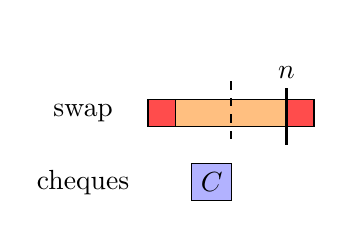
\begin{tikzpicture}
\node (middle)[draw, rectangle, fill=orange!50, minimum height=1em, minimum width=4em]{};
\node (leftred) [draw, rectangle, fill=red!70, minimum height=1em, minimum width=1em, node distance=2.5em, left of=middle]{};
\node (rightred)[draw, rectangle, fill=red!70, minimum height=1em, minimum width=1em, node distance=2.5em, right of=middle]{};
\node (zero) [above of=middle,node distance=2em, text height=1em] {};
\node (zerod) [below of=zero, node distance=3.5em] {};
\node (balance) [right of=zero,node distance=2em, text height=1.5em] {$n$};
\node (balanced) [below of=balance,node distance=3.5em] {};
\draw [dashed](zero)--(zerod);
\draw [very thick](balance)--(balanced);
\node (payment) [below of=zerod, node distance=1em]{};
\node (cheqeue) [draw, left of=payment, node distance=.7em, minimum height=1em, minimum width=1.4em, fill=blue!30, rectangle]{$C$};

\node (swap) [left of=leftred,minimum width=1em,align=right]{swap};
\node (cheques) [below of=swap,minimum width=1em, node distance= 2.5em, align=right]{cheques};
\end{tikzpicture}
&
\begin{tabular}{c}
  $\Longrightarrow$
\\ \\ \\ \\
\end{tabular}
&
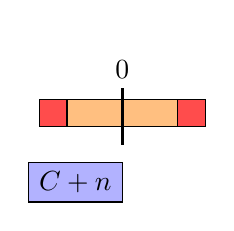
\begin{tikzpicture}
\node (middle)[draw, rectangle, fill=orange!50, minimum height=1em, minimum width=4em]{};
\node (leftred) [draw, rectangle, fill=red!70, minimum height=1em, minimum width=1em, node distance=2.5em, left of=middle]{};
\node (rightred)[draw, rectangle, fill=red!70, minimum height=1em, minimum width=1em, node distance=2.5em, right of=middle]{};
\node (zero) [above of=middle,node distance=2em, text height=1.5em] {$0$};
\node (zerod) [below of=zero, node distance=3.5em] {};
% \draw [dashed](zero)--(zerod);
\draw [very thick](zero)--(zerod);
\node (payment) [below of=zerod, node distance=1em]{};
\node (cheque) [draw, left of=payment, node distance=1.7em, minimum height=1em, minimum width=3.4em, fill=blue!30, rectangle]{$C+n$};
\end{tikzpicture}
\end{tabular}
\end{center}

\caption{Peer B's swap balance (with respect to A) reaches the payment threshold $n$ (left),
B sends a cheque to peer A. B keeps the cheque and restores the swap balance to zero.}
\label{fig:chequeswap}
\end{figure}
\end{center}

\subsection{Cancelling Cheques}

If the imbalance in the swap channel is the result of high variance as opposed to unequal consumption, after a period of accumulating cheques the channel balance starts tilting the other way. Normally it is now up to the other party to issue cheques to its peer resulting in uncashed cheques accumulating on both sides.
To allow for further savings in transaction costs, it could be desirable to be able to `play the cheques off against each other'.

Such a process is possible, but it requires certain deep changes within the chequebook contract. In particular, cashing cheques can no longer be immediate and must incur a security delay, familiar to anyone who has studied other implementations of payment channels.

Let us imagine a system analogous to cheques being returned to the issuer.  
Assume peer A issued cheques to B and the balance was brought back to zero. Later the balance tilts in A's favour but the cheques from A to B have not been cashed. In the real world, user B could simply return the last cheque back to A. In our case it is not so simple; we need some other mechanism by which B commits not to cash that particular cheque. Such a commitment could take many forms; it could be implemented by B signing a message allowing A to issue a new `last cheque` which has a lower cumulative total amount than before, or perhaps B can issue some kind of `negative` cheque for A's chequebook.

What all the implementations have in common, is that the chequebook can no longer allow instantaneous cashing of cheques. Upon receiving a cheque cashing request, the contract must wait to allow the other party in question to submit potentially missing information about cancelled cheques or reduced totals. 

We describe one possible implementation below.

\subsubsection{Waiving debt: bidirectional payments using a single chequebook }\label{subsubsec:waivingdebt}

To accommodate (semi-)bidirectional payments using a single chequebook we make the following modifications

\begin{enumerate}
    \item All cheques from user A to user B must contain a serial number.
    \item Each new cheque issued by A to B must increase the serial number.
    \item A's chequebook contract records the serial number of the last cheque that B cashed.
    \item During the cashing delay, valid cheques with higher serial number supersede any previously submitted cheques regardless of their face value.
    \item Any submitted cheque which decreases the payout of the previously submitted cheque is only valid if it is signed by the beneficiary.
\end{enumerate}

With these rules in place it is easy to see how cheque cancellation would work. 


Suppose user A has issued cheques $c_0 \ldots c_n$ with cumulative totals $t_0 \ldots t_n$ to user B. Suppose that the last cheque B cashed was $c_i$. The chequebook contract has recorded that B has received a payout of $t_i$ and that the last cheque cashed had serial number $i$.

Let us further suppose that the balance starts tilting in A's favour by some amount $x$. If B had already cashed cheque $c_n$, then B would now have to issue a cheque of her own using B's chequebook as the source and naming A as the beneficiary. However, since cheques $c_{i+1} \ldots c_n$  are uncashed, B can instead send to A a cheque with A's chequebook as the source, B as the beneficiary, with serial number $n+1$ and cumulative total $t_{n+1} = t_n - x$. Due to the rules enumerated above, A will accept this as equivalent to a payment of amount $x$ by B.

This process can be repeated multiple times until the cumulative total is brought back to $t_i$. At this point all outstanding debt has effectively been cancelled and any further payments must be made in the form of a proper cheque from B's chequebook to A.


\textbf{Suggestion - delete the rest of this subsection.}


In this scenario, instead of sending a cheque to A, B can waive part of their entitlement. This justifies swap as \emph{send waiver as payment} (see figure \ref{fig:waiverswap}).
A waiver essentially implements a proof that a cheque is destroyed and cannot be cashed, i.e., a promise that (part of) an uncashed cheque will not be redeemed.

A \gloss{waiver} is implemented as a note signed by the peer holding uncashed cheques %. The note specifies the current \gloss{swap index} (sequential number) 
 and indicates the amount of debt they agree to waive from their entitlement.

% \subsubsection*{Cashing cheques in the context of waivers}
If a channel is set to issue waived cheques then cashing must be a two step process.
Upon receiving a cheque, the contract verifies the data, and %signature and checks if the swap index matches the one on the cheque.
if the cheque is valid, the claimed amount is stored in a variable along with a timestamp. At this point a grace period starts: the original issuer gets notified of the cashing request and is invited to send in their last (highest) waiver signed by their peer. In case waivers are allowed cheques specify a \gloss{swap cycle index} and the contract keeps track of this.

% \subsubsection*{Cashing waivers}
Analogously to cheques, waivers are accepted by the contract. %if sent in as data in a transaction together with the issuer's address.
Upon receiving a waiver the contract verifies the data, and checks if the swap cycle index matches the one in the waiver.
If the waiver is valid, the peer's cumulative cashed balance is increased by the waived amount pretending the waived amount was paid out. Then the new cumulative cashed balance is compared to the one recorded when the cheque was received. Any remaining positive balance is transferred to the beneficiary, the cumulative sum is cleared from storage and the swap cycle index is incremented.

%%I stop here for now because the use of 'the swap index'  is confusing and I will rewrite it later ot be more clear.... a sequential index of waivers, stored by the checkbook separately from the serial number of the cheques but functioning like... how should this work? unclearly written

During the grace period the amount is not checked against the book's global balance.
After the grace period expires and no waiver was received, a second transaction
increments the swap cycle index and simply releases the funds or defaults on its debt.
During the grace period, further cheques can be sent to the contract: if they are valid and have the same swap cycle index as the one currently recorded, they simply replace the earlier one and the grace period is renewed.
Since waivers need to match the swap cycle index set by the cheques they destroy, they cannot be sent to the contract before the cheques they waive or after a new swap cycle starts.

In normal operation, however, peers are not incentivised to send in cheques as long as they can issue waivers. Once the waiver goes over the total amount of uncashed cheques, the peer needs to send a cheque. The swap cycle index is incremented in this cheque and the basis for issuing is the channel balance stored on the chain. This makes sure that cheques and waivers cannot be reused.%
%
\footnote{The volume of cheques waived will not increase the cumulative balance and therefore do not count toward total business volume for the purposes of credit history.
This can be amended if cheques are sent together with the latest waivers
and after validation the contract would adjust the cumulative balance to reflect the total volume.}

Using waivers can substantially increase the tolerated variance in the channel balance
without requiring actual transfer or impacting liquidity of the chequebook.
Without it, both peers would need to issue cheques and settlement would involve
transferring back and forth between the two peers, which means the first amount cashed
would not be available for a party for a period.

Waived cheques represent stronger guarantees since the cheque can effectively serve
as backing for incurring costs dedicated to the original issuer.

To summarise, Swap is ideally suited for immediately verifiable, recurring micropayments for bidirectional
services. The primary use case is bandwidth compensation and accounting to incentivise
relaying in a peer-to-peer system. As two peers are doing continuous business
they swap services, cheques and waivers and keep accounting and compensation offchain.




\begin{center}
\begin{figure}
\begin{center}
\begin{tabular}{ccc}
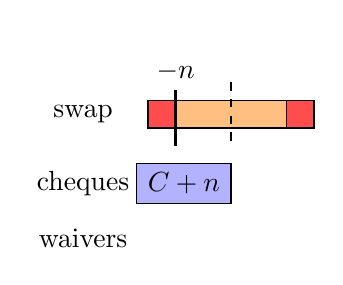
\begin{tikzpicture}
\node (middle)[draw, rectangle, fill=orange!50, minimum height=1em, minimum width=4em]{};
\node (leftred) [draw, rectangle, fill=red!70, minimum height=1em, minimum width=1em, node distance=2.5em, left of=middle]{};
\node (rightred)[draw, rectangle, fill=red!70, minimum height=1em, minimum width=1em, node distance=2.5em, right of=middle]{};
\node (zero) [above of=middle,node distance=2em, text height=1em] {};
\node (zerod) [below of=zero, node distance=3.5em] {};
\node (balance) [left of=zero,node distance=2em, text height=1.5em] {$-n$};
\node (balanced) [below of=balance,node distance=3.5em] {};
\draw [dashed](zero)--(zerod);
\draw [very thick](balance)--(balanced);
\node (payment) [below of=zerod, node distance=1em]{};
\node (cheque) [draw, left of=payment, node distance=1.7em, minimum height=1em, minimum width=3.4em, fill=blue!30, rectangle]{$C+n$};

\node (swap) [left of=leftred,minimum width=1em,align=right]{swap};
\node (cheques) [below of=swap,minimum width=1em, node distance= 2.5em, align=right]{cheques};
\node (waivers) [below of=cheques,minimum width=1em, node distance= 2em, align=right]{waivers};
\end{tikzpicture}
&
\begin{tabular}{c}
  $\Longrightarrow$
\\ \\ \\ \\
\end{tabular}
&
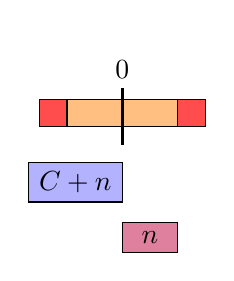
\begin{tikzpicture}
\node (middle)[draw, rectangle, fill=orange!50, minimum height=1em, minimum width=4em]{};
\node (leftred) [draw, rectangle, fill=red!70, minimum height=1em, minimum width=1em, node distance=2.5em, left of=middle]{};
\node (rightred)[draw, rectangle, fill=red!70, minimum height=1em, minimum width=1em, node distance=2.5em, right of=middle]{};
\node (zero) [above of=middle,node distance=2em, text height=1.5em] {$0$};
\node (zerod) [below of=zero, node distance=3.5em] {};
% \draw [dashed](zero)--(zerod);
\draw [very thick](zero)--(zerod);
\node (payment) [below of=zerod, node distance=1em]{};
\node (cheque) [draw, left of=payment, node distance=1.7em, minimum height=1em, minimum width=3.4em, fill=blue!30, rectangle]{$C+n$};
\node (waivers) [below of=payment, node distance=2em]{};
\node (waiver) [right of=waivers,minimum width=2em, node distance=1em,rectangle,draw,fill=purple!50]{$n$};
\end{tikzpicture}
\end{tabular}
\end{center}

\caption{Peer A's swap balance (with respect to B) reaches the payment threshold $n$ (left),
A sends a waiver to peer B. B keeps the waiver and restores the swap balance to zero}
\label{fig:waiverswap}
\end{figure}
\end{center}




\subsection{Payment channels}

If the variance is expected to be higher than the loss a peer can afford,
risk of insolvency can be mitigated by assigning part of the balance to a beneficiary.
This locked up sum, called \gloss{channel deposit} allows the owner a tilted balance and
serves as assured collateral dedicated to a particular peer.
This can be implemented by keeping peer-specific balances in the chequebook contract.
This deposit is no longer pooled over multiple creditors
and locking it can guarantee successful cashing of cheques up to the deposited amount.
Withdrawal from the channel deposit is possible but involves a grace period during which
the counterparty is invited to challenge the current balance by sending in the (last) cheque
with the highest amount. After the grace period the owner can reduce the deposit to cover only
its actual debt and may withdraw the remainder.
In order to get the balance of account between peers, the contract needs access to the counterparty
chequebook contract. For ease of explanation we assume that beneficiary is the
chequebook contract itself. Channel deposits can then be implemented as a map with beneficiary contract
address as key and the integer balance in wei as value.

Two chequebook contracts that have a record for each other constitute what is
called a \gloss{payment channel}.


\begin{center}
\begin{figure}
\begin{center}
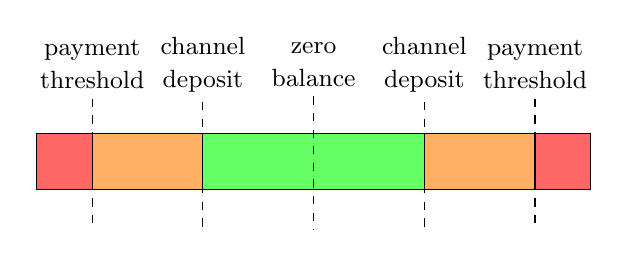
\begin{tikzpicture}
  \node (middle)[draw, rectangle, fill=green!60, minimum height=2em, minimum width=8em]{};
  \node (midleft)[draw, rectangle, fill=orange!60, minimum height=2em, minimum width=4em, node distance=6em, left of=middle]{};
\node (midright)[draw, rectangle, fill=orange!60, minimum height=2em, minimum width=4em, node distance=6em, right of=middle]{};
\node (leftred) [draw, rectangle, fill=red!60, minimum height=2em, minimum width=2em, node distance=9em,left of=middle]{};
\node (rightred)[draw, rectangle, fill=red!60, minimum height=2em, minimum width=2em, node distance=9em,right of=middle]{};
\node (zero) [above of=middle,node distance=3.5em, text width=4em, align=center] {\small zero\\ balance};
\node (zerod) [below of=middle] {};
\draw [dashed](zero)--(zerod);
\node (rtol) [node distance=8em,right of=zero,text width=4em, align=center] {\small payment\\threshold};
\node (rtold) [node distance=8em,right of=zerod] {};
\node (ltol) [node distance=8em,left of=zero,text width=4em, align=center] {\small payment\\threshold};
\node (ltold) [node distance=8em,left of=zerod] {};
\node (prtol) [node distance=4em,right of=zero,text width=4em, align=center] {\small channel\\deposit};
\node (prtold) [node distance=4em,right of=zerod] {};
\node (pltol) [node distance=4em,left of=zero,text width=4em, align=center] {\small channel\\deposit};
\node (pltold) [node distance=4em,left of=zerod] {};
\draw [dashed](rtol)--(rtold);
\draw [dashed](ltol)--(ltold);
\draw [dashed](prtol)--(prtold);
\draw [dashed](pltol)--(pltold);
\end{tikzpicture}
\end{center}
\caption{}
\label{fig:paymentchannel}
\end{figure}
\end{center}

\subsection{Zero cost entry}

An additional advantage of this construct is that one can start providing service with zero ether.
Since swap can also work only one way, if a party enters the system with zero ether (
gloss{newcomer}), but connects to peers with funds (\gloss{insider}), first they just provide the service (and not use it)
in order to produce a positive balance. In the simplest case insiders pay the newcomer on chain
but there are more efficient ways of bootstrapping.

If a newcomer connects to  an insider with an existing chequebook contract,
the insider agrees to create a chequebook contract for the newcomer
in return for consuming newcomers services.
 When insider's service debt reaches the amount needed by for contract creation,
 insider just sends a transaction to create the contract with newcomer as the owner.
Once a node has its own chequebook contract, they are able
to consume and potentially pay out more to their creditor.

In order to use the contract, however, it makes sense to have a balance on it.
Since the owner has no ether, it makes sense
to expect that the insider peers with funds will be the ones who deposit this starting balance.
If peers agreed that they want to save on transaction costs, it is reasonable to create
the contract with the required initial balance in one go. This would imply waiting out
with contract creation until the insider's debt reaches the \emph{cost of bootstrapping} which is
the sum of (1) the cost of contract creation, (2) the required starting balance, and (3) some
extra service fee to incentivises insiders to lend.

With the global deposit included, this cost of bootstrapping
can be substantially higher than nodes' loss tolerance.
If the contract is deployed to the blockchain in advance, with ownership granted
to the newcomer, the newcomer can just move with their new topped-up wallet
to other peers leaving the lender node with loss.
If it is to be deployed only after newcomer provided service totalling
the cost, then the insider node will disappear after essentially leeching on
the newcomer.

Luckily, there is a safe protocol to tackle
bootstrapping: the newcomer issues a cheque to the insider in advance with an amount
corresponding to the bootstrapping cost. Insider creates a contract with herself as owner
and a channel deposit also dedicated to herself in the amount
on the cheque. At this point if the two peers never meet, the newcomer suffered no loss,
the insider can just offer the contract to the next newcomer. Otherwise the service goes
exactly the way as if the newcomer was an insider with a contract, and the insider held
non-cashed cheques, i.e., as the insider consumes, each time it reaches the
payment threshold, it issues waivers against the withheld cheques. This is equivalent
to the insider setting up a subscription with newcomer, authorising withdrawal
with the waivers (see figure \ref{fig:bootstrapping}).

\begin{center}
\begin{figure}
\begin{center}
\end{center}
\caption{Bootstrapping or how to lauNch as a swap capable node consuming and providing a
service  and earn money}
\label{fig:bootstrapping}
\end{figure}
\end{center}


As newcomer provides service and insider issues waivers, it is business as usual.
Newcomer provides service to other peers and accepts payments sent to the
contract. If the inpayments are insufficient to get the balance up
to cover the bootstrapping cost, the entire contract is still owned by the insider
who can reuse it with another peer with previous inpayments counting as profit.
In this case neither the cheque nor the waivers are valid, therefore all the service insider
may have received was free.

If the balance goes above the cost of bootstrapping, the insider can cash it with
the original cheque which will automatically change the owner to newcomer.
The cheque works exactly as normal, i.e., when cashed, it is stored in escrow
while the contract receive waivers.
Waivers can be used to first cover the difference between channel deposit and balance, and above that
count to reduce the outpayment to insider. In normal operation, once waivers goes over
the cost of bootstrapping, insider issues ???

This system is complete if newcomers have a way to send waivers to the contract.
Since newcomers have zero balance, they cannot bear the transaction   cost and need others to send it for them. 
Waivers and cheques can be signed by their beneficiary. These variants are also accepted by the chequebook
and instruct the contract to pay an amount to the transaction sender covering the transaction cost plus a small service fee.  This way the prospect of the bounty serves as an incentive to
third party insiders to transact on behalf of newcomers.
The waiver or cheque triggers outpayment from the chequebook global  balance to the owner.
This is how to earn ether with a service starting from nothing in the most efficient way.
Signed notes are not only useful for newcomers; anyone without a blockchain connection
will be able to interact and provide services without losing the security of the blockchain.

To summarise, by serving before consuming, participants can
bootstrap their way into swap without the need for funds.
Hence swap is justified as (\emph{setting up a wallet as payment}).
